\section{Experimental Protocol}
\subsection{Development map and confirmation selection}
The study's primary estimand is the difference in diagnostic admission at development-selected boundaries, not global recovery performance. A deterministic map evaluates seven standard-deviation scales $\{.25,.5,.75,1,1.25,1.5,2\}$, four log-gain decline bounds $\{0,.045,.09,.15\}$~s$^{-1}$ and 241 measured power/sensitivity ratios from 1 to 2.2 in increments .005. All 6,748 points are retained. The map uses a measured zero angle to isolate admission geometry and is not a causal plant simulation.

Before the original confirmation outcomes, the protocol chooses the lexicographically first noise/bound group with each disagreement direction, the midpoint of its band and adjacent below/above controls. This representative-band choice is a disclosed narrowing from an initial proposal to confirm every transition. Both directions and all controls are retained. Region~1 has noise scale .25, $\ell=0$, and power ratios 1.905, 1.990, 2.075. Region~2 has scale .75, $\ell=0$, and ratios 2.175, 2.1875, 2.200. Thus $\sigma_q$ is .02 or $.06\um$, $\sigma_v$ is .04 or $.12\um$/s, and $\sigma_p$ is .002 or .006. Low noise and nondeclining gain are stronger assumptions than in the preserved drift benchmark.

The map's measured ratio is translated into a post-change physical gain $g=({\rm ratio})p_{\min}/p_0$. Gain is initially one and changes at $t=2$~s to that constant level. Actual boresight offset is zero. The link is usable in these tests, so subsequent evidence acquisition earns no recovery credit. State is initialized at zero. The causal trigger requires three consecutive samples with absolute log residual exceeding .18, after $t>1$~s; the residual uses measured angle/power and nominal optics. Decisions have no true fault label, true offset or actual mismatch as input.

\subsection{Methods and matched resource conditions}
The original confirmation compares the uncertainty-aware diagnostic selector (UAD, labeled ``Certificate'') with a fixed-$2\um$ guard. The guard retains the same starting-power interval, centered optical bound, information check, cost and offline constraint checks, but substitutes $2\um+\epsilon_q$ for the delivered-motion radius. It is an explicitly heuristic margin, not a proven enclosure. Both select balanced eight-dwell candidates with a 2.88-s excitation limit.

An additional protocol is frozen after the original selector outcomes are known, but before any new baseline outcome. It evaluates parameter KF and conventional extremum seeking at the identical six settings, seeds, six actual models, Gaussian disturbances, trigger and 2.88-s time limit. This extension is exploratory; the four methods were not jointly predeclared before the original confirmation. Source hashes and both protocols preserve the sequence.

The parameter filter uses a four-state transformed model: two offset coefficients, a current nuisance intercept and a log-gain slope. Sequential linear updates use first-order angle/power variance, Joseph covariance updates and process tuning zero. Its fixed diagnostic waveform has $6\um$ amplitude and eight .36-s dwells. It has no service certificate. The ES tracker uses $4\um$ sinusoidal dither at .25/.4~Hz, unit-rate washout, demodulation, .7-rate gradient filtering and adaptation gain .3. It reports tracking/correction outcomes, not a diagnostic fit. These tunings are inherited from disjoint development seeds 41--45 and were not retuned on extension outcomes. The short window is less than a full period of its slow sinusoid; native-duration tracking behavior is therefore considered separately in the supplement.

All methods use the common nominal PID, physical torque/rate/command constraints and measured information boundary. Equal time does not imply equal realized angular energy or equal diagnostic objectives. The filter's larger waveform and absence of service refusal are explicit differences; observed success does not certify an unsafe trajectory, nor does a missing certificate itself demonstrate failure. The original source's finite-horizon behavior is retained: a probe triggered too late can be incomplete at 14~s. Such records have no completed fit and are counted separately rather than forced into rejection.

\subsection{Seeds, endpoints and paired statistics}
For each setting and method, seeds 7001--7100 are paired across all six actual actuator pairs. Each two-method study contains $6\times100\times6\times2=7,200$ runs; together they contain 14,400, with 600 records per setting/method. Reusing common random numbers couples the comparisons without treating six fixed model outputs as independent random subjects.

The protocol records selection/authorization, completed-fit acceptance, approximate-confidence misses, sampled mission and probe-induced outage, angular excitation $h\sum_{k\in\mathrm{probe}}\norm{q_k}^2$, and certificate slack. Angular excitation is reported in $\mu$rad$^2$~s and is not electrical energy. Slack is the per-trace median $(p-\underline p)/p_{\min}$, summarized across selected traces. Incompletion is an additional finite-horizon accounting endpoint exposed by the new replay audit; historical per-run values are unchanged.

Paired differences average the six fixed-model contrasts within each seed, then resample the 100 seed units 5,000 times. Percentile 95\% intervals and approximate Bonferroni percentile limits over six settings are supplied. Adjustment is separately scoped per comparator and outcome; it does not cover every endpoint jointly and is not an exact small-sample confidence guarantee. ES receives no fit-acceptance comparison because it has no estimator output. The complete rows and intervals are supplied rather than selecting only favorable comparisons.

\subsection{Evidence categories and independent calculation}
Each new trace retains pre-step eight-state history, next held reference, final state, all standardized disturbances, true offset/gain, actual and measured power/angle, commanded torque, candidate bound and fit. New baseline traces additionally label the rate units explicitly. Separate NumPy code reconstructs optical power, trigger timing, metrics and each RK4 step including stage saturation and anti-windup. This checks the same sampled model independently; it does not physically replicate it.

A calculated UAD bound is ``within-premise'' when all required histories exist and numeric premise checks pass under the declared simulator. A known failed premise gives ``out-of-model'' precedence; otherwise missing required histories give ``unverified.'' Noncertificate baselines are not relabeled certified just because no outage occurs. Distributional calibration and model truth remain assumptions even for a within-premise record. Sensitivity evidence, earlier incomplete histories and corrected historical statistical exports belong to a separate evidence category documented in the supplement, rather than enlarging the confirmation denominator.

\begin{figure*}[t]
\centering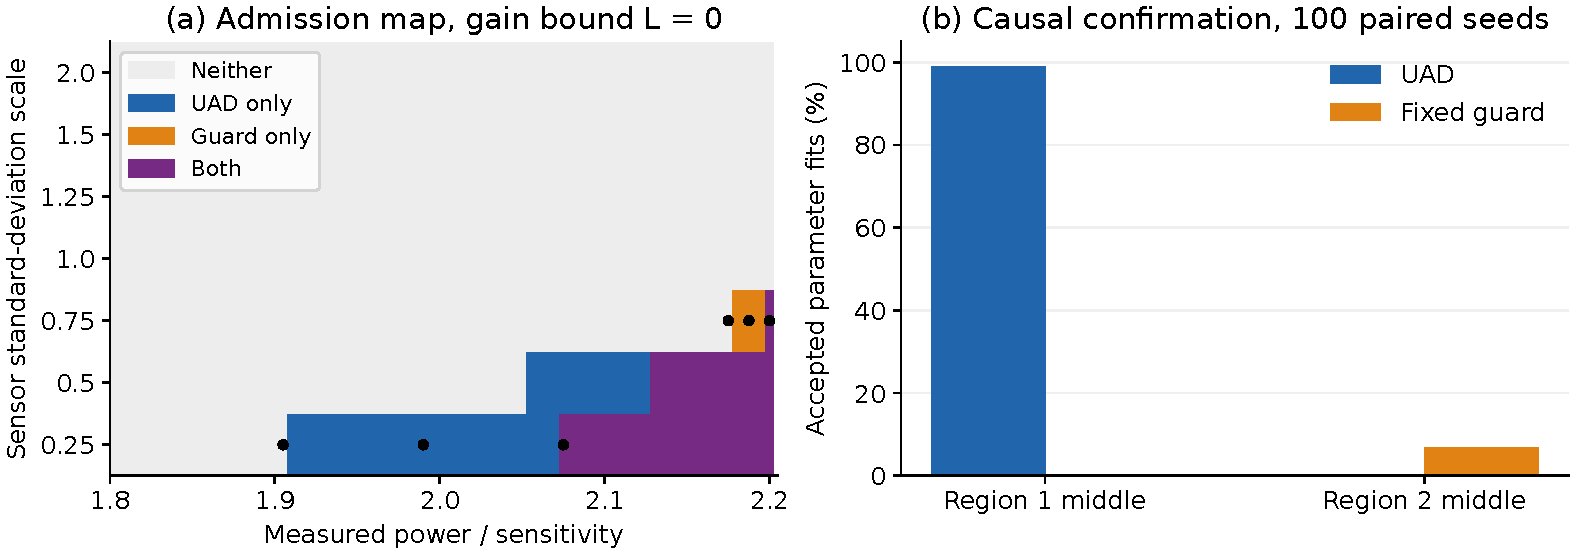
\includegraphics[width=.96\textwidth]{admission_confirmation.pdf}
\caption{Preserved development-map zoom and original two-selector midpoint confirmation. All six chosen settings are marked, including the controls; the full 6,748-point map is supplementary. The right panel concerns accepted fits only. The additional filter/ES extension is shown separately in Fig.~\ref{fig:matched}.}
\label{fig:frontier}
\end{figure*}
